\documentclass[12pt, a4paper]{article}

% =============================================================================
% PAQUETES BÁSICOS
% =============================================================================
\usepackage[spanish]{babel} % Soporte para español
\usepackage[utf8]{inputenc}   % Codificación de entrada
\usepackage[T1]{fontenc}      % Codificación de fuentes

% =============================================================================
% PAQUETES DE ESTILO Y DISEÑO
% =============================================================================
\usepackage[svgnames]{xcolor} % Para usar colores (ej. SteelBlue, DarkGray)
\usepackage{graphicx}         % Para incluir imágenes
\usepackage[a4paper, margin=2.5cm, top=3cm, bottom=3cm]{geometry} % Márgenes

\usepackage{titlesec}         % Alternativa moderna para estilizar títulos
\usepackage{url}              % Para formatear URLs
\usepackage{enumitem}         % Para personalizar listas

% =============================================================================
% PAQUETES ACADÉMICOS Y MATEMÁTICOS
% =============================================================================
\usepackage{amsmath}
\usepackage{amsfonts}
\usepackage{amssymb}
\usepackage{booktabs} % Para tablas de calidad profesional
\usepackage{float}      % Para control de flotantes [H]
\usepackage{array}      % Para tablas más complejas
\usepackage{longtable}  % Para tablas que ocupan más de una página
\usepackage{adjustbox}  % Para ajustar el tamaño de tablas/imágenes
\usepackage{caption}    % Para personalizar captions
\usepackage{subcaption} % Para subfiguras y subtables (reemplaza subfig)
\usepackage{cite}       % Para gestionar citaciones
\usepackage{multirow}   % Mantenemos este paquete del documento original

% =============================================================================
% CONFIGURACIÓN DE COLORES Y ESTILOS
% =============================================================================
% Colores Institucionales USACH (basados en el tema de la presentación)
\definecolor{usachBlue}{RGB}{0, 47, 108}
\definecolor{usachGray}{RGB}{177, 177, 177}

% --- Estilo de Títulos de Sección ---
% Formato para \section
\titleformat{\section}
  {\normalfont\Large\bfseries\color{usachBlue}}  % Estilo
  {\thesection}                                    % Etiqueta (numeración)
  {1em}                                            % Espacio horizontal
  {}                                               % Código antes del título
  
% Formato para \subsection
\titleformat{\subsection}
  {\normalfont\large\bfseries\color{usachBlue!80!black}}  
  {\thesubsection}
  {1em}
  {}
  
% Formato para \subsubsection
\titleformat{\subsubsection}
  {\normalfont\normalsize\bfseries\color{usachBlue!60!black}}
  {\thesubsubsection}
  {1em}
  {}

\usepackage{tcolorbox}
\tcbuselibrary{skins}
\usepackage{tikz}
\usepackage{hyperref}

% --- Configuración de Hyperref ---
\hypersetup{
    colorlinks=true,
    linkcolor=usachBlue,
    filecolor=usachBlue,      
    urlcolor=usachBlue,
    citecolor=usachBlue!80!black,
    pdftitle={Resolución del QAP mediante Búsqueda Tabú},
    pdfauthor={Camila Llamirez, Pablo Jordan, Camilo Avendaño},
    pdfkeywords={QAP, Búsqueda Tabú, Metaheurísticas, Optimización},
    bookmarks=true,
    bookmarksopen=true
}

% --- Metadatos del Documento ---
\title{Resolución del Problema de Asignación Cuadrática mediante Búsqueda Tabú}
\author{Camila Llamirez, Pablo Jordan, Camilo Avendaño}
\date{13 de Junio de 2025} % Fecha específica como en la portada de b.tex

% Configuración global de leyendas (caption) para subcaption
\captionsetup{font=small,labelfont=bf}

% =============================================================================
% INICIO DEL DOCUMENTO
% =============================================================================
\begin{document}

% --- Portada Personalizada ---
\begin{titlepage}
    % Fondo y márgenes
    \pagecolor{white}
    
    % Encabezado institucional
    \begin{center}
        
\includegraphics[height=2.5cm]{logo_usach.png} % Logo USACH más grande
        \vspace{0.5cm} % Adjusted
        
        {\large\bfseries\textsc{\textcolor{usachBlue}{Universidad de Santiago de Chile}}} \\
        {\large\textsc{Facultad de Ingeniería}} \\
        {\large\textsc{Departamento de Ingeniería Informática}} \\
    \end{center}
    
    % Separador decorativo
    \vspace{0.0pt} 
    \begin{center}
        \textcolor{usachBlue}{\rule{0.8\textwidth}{1pt}} 
    \end{center}
    \vspace{0.0pt} 
    
    % Título principal con marco
    \begin{center}
        \begin{tcolorbox}[
            enhanced,
            colback=white,
            colframe=usachBlue,
            arc=0mm,
            boxrule=1.5pt,
            left=10pt,right=10pt,top=12pt,bottom=12pt,
            boxsep=0pt,
            width=0.95\textwidth
        ]
            \centering
            {\Huge \bfseries \textcolor{usachBlue}{Resolución del Problema de}} \\
            {\Huge \bfseries \textcolor{usachBlue}{Asignación Cuadrática}} \\
            {\Huge \bfseries \textcolor{usachBlue}{mediante Búsqueda Tabú}} \\
        \end{tcolorbox}
    \end{center}
    
    % Subtítulo
    \vspace{1.0cm} 
    \begin{center}
        {\Large\bfseries Trabajo Final Unidad II}\
    \end{center}
    \vspace{2cm} 
    
    % Información del curso - REVISED BLOCK
    \begin{center}
    \large % Make text in this block large
    \begin{tabular}{l@{\hspace{2em}}l} 
        \textbf{Autores:} & \begin{tabular}[t]{@{}l@{}}Camila Llamirez \\ Pablo Jordan \\ Camilo Avendaño\end{tabular} \\[1.2em]
        \textbf{Asignatura:} & \begin{tabular}[t]{@{}l@{}}Algoritmos Avanzados \\ y Complejidad Computacional\end{tabular} \\[1.2em]
        \textbf{Profesor:} & Mario Inostroza 
    \end{tabular}
    \end{center}
    
    % Pie de página
    \vfill
    \begin{center}
        \textcolor{usachBlue}{\rule{0.4\textwidth}{0.8pt}} \\
        \vspace{0.3cm} 
        {\large Santiago, 13 de Junio de 2025} 
    \end{center}
\end{titlepage}

% --- Índices ---
\newpage
\tableofcontents
\newpage

% =============================================================================
\section{Introducción}
% =============================================================================

El Problema de Asignación Cuadrática (QAP) representa uno de los desafíos fundamentales en la optimización combinatoria, siendo clasificado como NP-hard \cite{sahni1976}. Su importancia trasciende el ámbito teórico, con aplicaciones críticas en el diseño de instalaciones industriales \cite{koopmans1957}, la arquitectura de circuitos VLSI \cite{steinberg1961}, el diseño de teclados ergonómicos \cite{burkard1997}, y más recientemente en bioinformática computacional para el análisis de interacciones proteína-proteína \cite{anstreicher2003}. Dada su complejidad, el uso de metaheurísticas se presenta como el enfoque más efectivo para obtener soluciones de alta calidad en tiempos de cómputo razonables.

El objetivo principal de este estudio es implementar y evaluar el rendimiento de la metaheurística de \textbf{Búsqueda Tabú (Tabu Search)} para resolver un conjunto de instancias de referencia del QAP. La elección de esta técnica se fundamenta en su demostrada robustez para guiar la exploración del espacio de soluciones y evitar óptimos locales mediante el uso de estructuras de memoria.

Para la experimentación, se utilizará un conjunto de 8 instancias clásicas extraídas de la librería QAPLIB \cite{burkard1997qaplib}, una colección estándar para la validación de algoritmos. Estas instancias representan un espectro diverso de características y tamaños, lo que permitirá evaluar la escalabilidad y adaptabilidad del algoritmo. El desempeño se medirá en términos de la calidad de las soluciones obtenidas (comparadas con los valores óptimos o las mejores soluciones conocidas) y el tiempo de ejecución requerido.

Este informe se estructura de la siguiente manera: primero, se presenta una explicación formal del Problema de Asignación Cuadrática. A continuación, se describe en detalle la metaheurística de Búsqueda Tabú y el modelamiento del problema. Posteriormente, se exponen los resultados de las pruebas computacionales, tanto a nivel individual por instancia como de forma global. Finalmente, se presentan las conclusiones derivadas del estudio y se comentan posibles líneas de trabajo futuro.

\newpage

% =============================================================================
\section{Explicación del Problema de Asignación Cuadrática (QAP)}
% =============================================================================

\subsection{Definición Formal}

El Problema de Asignación Cuadrática fue introducido por Koopmans y Beckmann \cite{koopmans1957} como un modelo matemático para el problema de localización de plantas industriales. Formalmente, el QAP busca asignar un conjunto de $n$ facilidades a un conjunto de $n$ localizaciones, minimizando el costo total de transporte.

Dadas dos matrices:
\begin{itemize}
    \item $F = (f_{ij}) \in \mathbb{R}^{n \times n}$: matriz de flujos, donde $f_{ij}$ representa el flujo de materiales, información o interacción entre las facilidades $i$ y $j$
    \item $D = (d_{kl}) \in \mathbb{R}^{n \times n}$: matriz de distancias, donde $d_{kl}$ denota la distancia o costo de transporte entre las localizaciones $k$ y $l$
\end{itemize}

El objetivo es encontrar una permutación $\pi \in S_n$ (donde $S_n$ denota el grupo simétrico de orden $n$) que minimice:

\begin{equation}
\min_{\pi \in S_n} z(\pi) = \sum_{i=1}^{n} \sum_{j=1}^{n} f_{ij} \cdot d_{\pi(i)\pi(j)}
\label{eq:qap}
\end{equation}

\subsection{Complejidad Computacional}

La complejidad intrínseca del QAP se manifiesta en múltiples dimensiones:

\begin{table}[H]
\centering
\caption{Características de complejidad del QAP}
\begin{tabular}{@{}lp{8cm}@{}}
\toprule
\textbf{Aspecto} & \textbf{Descripción} \\
\midrule
Espacio de búsqueda & $n!$ permutaciones posibles, crecimiento factorial \\
Complejidad & NP-hard \cite{sahni1976}, no existe algoritmo polinomial conocido \\
Estructura & No lineal, multimodal, sin propiedades de convexidad \\
Evaluación & $O(n^2)$ operaciones por solución \\
Aproximación & No existe PTAS (Polynomial Time Approximation Scheme) \cite{arora1998} \\
\bottomrule
\end{tabular}
\end{table}

\subsection{Aplicaciones Prácticas}

El QAP modela numerosos problemas del mundo real:

\begin{enumerate}
    \item \textbf{Diseño de instalaciones}: Ubicación óptima de departamentos en hospitales \cite{elshafei1977}, fábricas \cite{taillard1995} y centros comerciales
    \item \textbf{Diseño electrónico}: Posicionamiento de componentes en circuitos VLSI para minimizar la longitud de conexiones \cite{steinberg1961}
    \item \textbf{Economía}: Análisis de flujos comerciales entre regiones \cite{krarup1978}
    \item \textbf{Bioinformática}: Predicción de estructura de proteínas y análisis de redes metabólicas \cite{phillips2000}
    \item \textbf{Procesamiento de imágenes}: Correspondencia de características en visión por computador \cite{maciel2003}
\end{enumerate}

\newpage

% =============================================================================
\section{Descripción de la Metaheurística: Búsqueda Tabú}
% =============================================================================

\subsection{Fundamentos Teóricos}

La Búsqueda Tabú (TS), introducida por Fred Glover \cite{glover1989, glover1990}, representa un paradigma de búsqueda inteligente que trasciende las limitaciones de los métodos de búsqueda local tradicionales mediante el uso sistemático de estructuras de memoria. A diferencia de métodos como hill climbing que terminan en el primer óptimo local, TS utiliza memoria adaptativa para continuar la exploración.

\subsection{Justificación de la Selección}

La elección de Búsqueda Tabú sobre otras metaheurísticas se fundamenta en un análisis comparativo exhaustivo de la literatura especializada en QAP:

\begin{table}[H]
\centering
\caption{Comparación de metaheurísticas para QAP basada en literatura}
\label{tab:comparacion_meta}
\adjustbox{width=\textwidth}{
\begin{tabular}{@{}lccccl@{}}
\toprule
\textbf{Metaheurística} & \textbf{Gap típico} & \textbf{Tiempo} & \textbf{Robustez} & \textbf{Complejidad} & \textbf{Referencias clave} \\
\midrule
Búsqueda Tabú & 1-5\% & Rápido & Alta & Media & \cite{taillard1991, battiti1994, drezner2005} \\
Recocido Simulado & 3-8\% & Medio & Media & Baja & \cite{connolly1990, wilhelm1987} \\
Algoritmos Genéticos & 5-10\% & Lento & Media & Alta & \cite{tate1995, drezner2003, ahuja2000} \\
ACO & 2-6\% & Muy lento & Media & Alta & \cite{stutzle2000, gambardella1999} \\
GRASP & 3-7\% & Medio & Alta & Media & \cite{li2000, oliveira2004} \\
VNS & 2-5\% & Medio & Alta & Media & \cite{mladenovic2007, hansen2004} \\
Híbridos GA+LS & 1-3\% & Lento & Alta & Muy alta & \cite{fleurent1994, merz2000} \\
\bottomrule
\end{tabular}
}
\end{table}

Los estudios comparativos de Cela \cite{cela1998} y Loiola et al. \cite{loiola2007} confirman que TS consistentemente produce soluciones de alta calidad con tiempos computacionales competitivos. Específicamente:

\begin{itemize}
    \item \textbf{Taillard \cite{taillard1991}}: Demostró que TS robusta alcanza gaps < 2\% en el 90\% de instancias QAPLIB
    \item \textbf{Battiti y Tecchiolli \cite{battiti1994}}: TS reactiva supera a SA en calidad y velocidad
    \item \textbf{James et al. \cite{james2009}}: TS cooperativa establece nuevos récords en instancias grandes
\end{itemize}

\subsection{Componentes Diferenciadores}

\subsubsection{Estructura de Memoria}

La memoria en TS se organiza en tres niveles \cite{glover1997}:

\begin{table}[H]
\centering
\caption{Niveles de memoria en Búsqueda Tabú}
\begin{tabular}{@{}lll@{}}
\toprule
\textbf{Tipo} & \textbf{Función} & \textbf{Implementación QAP} \\
\midrule
Corto plazo & Prevenir ciclos & Lista tabú de movimientos recientes \\
Medio plazo & Intensificación & Atributos de buenas soluciones \\
Largo plazo & Diversificación & Frecuencia de asignaciones \\
\bottomrule
\end{tabular}
\end{table}

\subsubsection{Lista Tabú}

Para QAP, la implementación eficiente utiliza una matriz $T \in \mathbb{N}^{n \times n}$ donde $T[i,j]$ indica hasta qué iteración está prohibido asignar la facilidad $i$ a la localización $j$ \cite{taillard1991}. El tenure (duración de la prohibición) es crítico:

\begin{itemize}
    \item \textbf{Tenure estático}: $\tau = \alpha \cdot n$, típicamente $\alpha \in [0.5, 1.5]$ \cite{taillard1991}
    \item \textbf{Tenure dinámico}: $\tau = \tau_{base} + \text{random}(-\delta, \delta)$ \cite{battiti1994}
    \item \textbf{Tenure reactivo}: Ajuste basado en detección de ciclos \cite{battiti1994}
\end{itemize}

\subsubsection{Criterio de Aspiración}

El criterio más efectivo para QAP es la aspiración por objetivo \cite{glover1989}:

\begin{equation}
\text{Movimiento }(i,j)\text{ permitido si } z(\pi') < z^* \text{ (mejor global)}
\end{equation}

Estudios empíricos \cite{taillard1995} muestran que este criterio simple supera a variantes más sofisticadas en QAP.

\subsubsection{Estrategias de Diversificación e Intensificación}

Basándonos en \cite{glover1997, gendreau2003}:

\begin{itemize}
    \item \textbf{Diversificación}:
    \begin{itemize}
        \item Penalización por frecuencia de uso \cite{kelly1995}
        \item Reinicios estratégicos preservando componentes élite \cite{james2009}
        \item Perturbación adaptativa basada en entropía \cite{battiti1994}
    \end{itemize}
    
    \item \textbf{Intensificación}:
    \begin{itemize}
        \item Reducción temporal del tenure en regiones prometedoras
        \item Path relinking entre soluciones élite \cite{glover2000}
        \item Búsqueda local exhaustiva en subvecindarios
    \end{itemize}
\end{itemize}

\newpage

% =============================================================================
\section{Modelamiento del Problema con la Metaheurística}
% =============================================================================

\subsection{Representación de la Solución}

Para el Problema de Asignación Cuadrática, una solución consiste en asignar cada una de las \(n\) instalaciones a una de las \(n\) localizaciones disponibles. La representación más natural y computacionalmente eficiente para una solución es un \textbf{array de permutación} \cite{burkard1998}.

Una solución \(\pi\) se representa como un vector de longitud \(n\), donde el elemento en la posición \(i\)-ésima, \(\pi(i)\), denota la localización a la que se asigna la instalación \(i\). Por ejemplo, para un problema con \(n=4\), la solución \(\pi = (3, 1, 0, 2)\) se interpreta de la siguiente manera:
\begin{itemize}
    \item La instalación 0 se asigna a la localización 3.
    \item La instalación 1 se asigna a la localización 1.
    \item La instalación 2 se asigna a la localización 0.
    \item La instalación 3 se asigna a la localización 2.
\end{itemize}
Esta representación es compacta y garantiza la factibilidad de la solución.

\subsection{Manejo de Restricciones}

El QAP posee dos restricciones fundamentales implícitas en su definición:
\begin{enumerate}
    \item Cada instalación debe ser asignada a una y solo una localización.
    \item Cada localización debe ser ocupada por una y solo una instalación.
\end{enumerate}
Una de las principales ventajas de utilizar una representación de permutación es que estas dos restricciones se cumplen inherentemente. Por definición, una permutación es una biyección, garantizando que cada instalación se asigna a una única localización y viceversa. Por lo tanto, no se requieren mecanismos adicionales de penalización o reparación, simplificando el diseño del algoritmo.

\subsection{Función Objetivo y Evaluación Incremental}

La función objetivo del QAP, que se busca minimizar, se evalúa como:
\begin{equation}
z(\pi) = \sum_{i=1}^{n} \sum_{j=1}^{n} f_{ij} \cdot d_{\pi(i)\pi(j)}
\end{equation}

Dado que la Búsqueda Tabú evalúa un gran número de soluciones vecinas en cada iteración, recalcular el costo completo ($O(n^2)$) es computacionalmente prohibitivo. Por ello, es fundamental implementar una \textbf{evaluación incremental} (o \textit{delta evaluation}) \cite{taillard1991}. Al intercambiar las asignaciones de dos facilidades, $a$ y $b$, el cambio en el costo ($\Delta$) se puede calcular en tiempo $O(n)$:

\begin{equation}
\Delta_{ab}(\pi) = \sum_{k \neq a,b} \left[ (f_{ak} - f_{bk})(d_{\pi(b)\pi(k)} - d_{\pi(a)\pi(k)}) + (f_{ka} - f_{kb})(d_{\pi(k)\pi(b)} - d_{\pi(k)\pi(a)}) \right]
\label{eq:delta}
\end{equation}

El nuevo costo de la solución $\pi'$ es entonces $z(\pi') = z(\pi) + \Delta_{ab}(\pi)$. Esta optimización es crucial para la eficiencia del algoritmo \cite{burkard1984}.

\subsection{Estructura de Vecindario}

Para el QAP, la estructura de vecindario más común y efectiva es la de \textbf{2-intercambio} (2-opt o swap) \cite{burkard1998}. El vecindario $N(\pi)$ de una solución $\pi$ se define como el conjunto de todas las soluciones que se pueden obtener intercambiando las asignaciones de exactamente dos facilidades. En la implementación, este vecindario se explora exhaustivamente mediante un doble bucle anidado que considera todos los pares de facilidades $i,j \in \{0,\dots,n-1\}$ con $i 
eq j$. La complejidad de explorar el vecindario completo es $O(n^2)$, pero gracias a la evaluación incremental del costo, el costo total por iteración se mantiene en $O(n^2)$.

El tamaño de este vecindario es $\frac{n(n-1)}{2}$. En la implementación, se utiliza un esquema de exploración sistemática que mantiene un registro de los mejores movimientos encontrados durante la exploración del vecindario. Esto permite implementar una estrategia de búsqueda mejorada que prioriza los movimientos más prometedores en la siguiente iteración.

\newpage

% =============================================================================
\section{Experimentación Computacional}
% =============================================================================

\subsection{Ambiente de Pruebas y Parámetros}

\paragraph{Hardware y Software de Experimentación.}
Los experimentos se llevaron a cabo en el siguiente entorno computacional:

\begin{center}
\begin{tabular}{ll}
\hline
\textbf{Componente} & \textbf{Especificación} \\
\hline
Procesador & Apple M4 Max \\
Memoria RAM & 128 GB Unificada \\
Sistema Operativo & macOS 15.5 \\
Lenguaje de Programación & Python 3 \\
Entorno de Desarrollo & PyCharm \\
Librerías Clave & NumPy \\
\hline
\end{tabular}
\end{center}

\paragraph{Configuración del Algoritmo de Búsqueda Tabú.}
Los parámetros clave de la Búsqueda Tabú implementada se configuraron de la siguiente manera:
\begin{itemize}
    \item \textbf{Criterio de detención:} Un máximo de 100,000 evaluaciones de la función objetivo.
    \item \textbf{Estructura de vecindario:} Se utiliza el vecindario completo basado en el operador de intercambio \textit{2-opt} (o \textit{swap}).
    \item \textbf{Tenencia Tabú:} Se ha fijado un valor de tenencia tabú estático en \textbf{20}.
    \item \textbf{Reproducibilidad:} Se utilizó una semilla aleatoria fija (\texttt{numpy.random.seed(42)}) para garantizar que los resultados sean completamente reproducibles.
\end{itemize}

\paragraph{Metodología de Ejecución y Recolección de Datos.}
Para cada instancia del problema, se realizaron \textbf{11} ejecuciones independientes del algoritmo de Búsqueda Tabú. El script principal, desarrollado en Python, automatiza este proceso y se encarga de:
\begin{itemize}
    \item Registrar los costos detallados de la solución encontrada en cada iteración para cada una de las 11 ejecuciones, almacenándolos en un fichero JSON (\texttt{results/per\_iteration\_costs.json}).
    \item Generar un resumen global de resultados agregados por instancia (mejor costo, costo promedio, desviación estándar, GAP, tiempo promedio), guardado en un fichero de texto (\texttt{results/summary.txt}).
    \item Crear gráficos de convergencia individuales para cada instancia, mostrando la evolución del costo a lo largo de las iteraciones para las 11 ejecuciones (\texttt{results/graphs/}).
\end{itemize}

\paragraph{Obtención de los Valores Óptimos de Referencia.} Para evaluar la calidad de las soluciones, es fundamental compararlas con la mejor solución conocida o el óptimo probado para cada instancia, obtenidos de QAPLIB. Para las instancias \textbf{esc32h} y \textbf{esc64a}, cuyos valores no se encontraban en los ficheros de solución, se utilizaron los óptimos documentados en el sitio web de QAPLIB (438 y 116 respectivamente), lo que permitió un cálculo homogéneo del \% GAP.

\newpage
\subsection{Resultados por Instancia}

A continuación, se presentan los resultados detallados para cada una de las 8 instancias. Cada gráfico muestra la convergencia del costo a lo largo de 11 ejecuciones independientes, permitiendo analizar tanto la calidad de las soluciones como la robustez del algoritmo en diferentes tipos de instancias.

\subsubsection{Instancia bur26c}
La instancia \texttt{bur26c} (n=26) presenta las siguientes características de rendimiento con la Búsqueda Tabú implementada:

\begin{itemize}
    \item \textbf{Calidad de Solución (Mejor GAP):} Se alcanzó un Mejor GAP del 0.16\%.
    \item \textbf{Calidad de Solución (GAP Promedio):} El GAP Promedio fue del 0.59\%.
    \item \textbf{Consistencia de Resultados:} La desviación estándar de los costos fue de 17468.91 (aproximadamente 0.32\% del costo promedio), indicando una alta consistencia.
    \item \textbf{Eficiencia Computacional:} El tiempo promedio de ejecución fue de 1.75s.
\end{itemize}

\textbf{Análisis del Comportamiento:}
El algoritmo demostró una convergencia rápida y estable para \texttt{bur26c}, encontrando consistentemente soluciones muy cercanas al óptimo conocido. La baja dispersión de los resultados sugiere un paisaje de búsqueda relativamente favorable.

\textbf{Conclusión Específica de la Instancia:}
La configuración actual de la Búsqueda Tabú se muestra altamente efectiva para la estructura de \texttt{bur26c}, permitiendo una exploración eficiente y la obtención de soluciones de alta calidad con notable rapidez.
\begin{figure}[H]
\centering
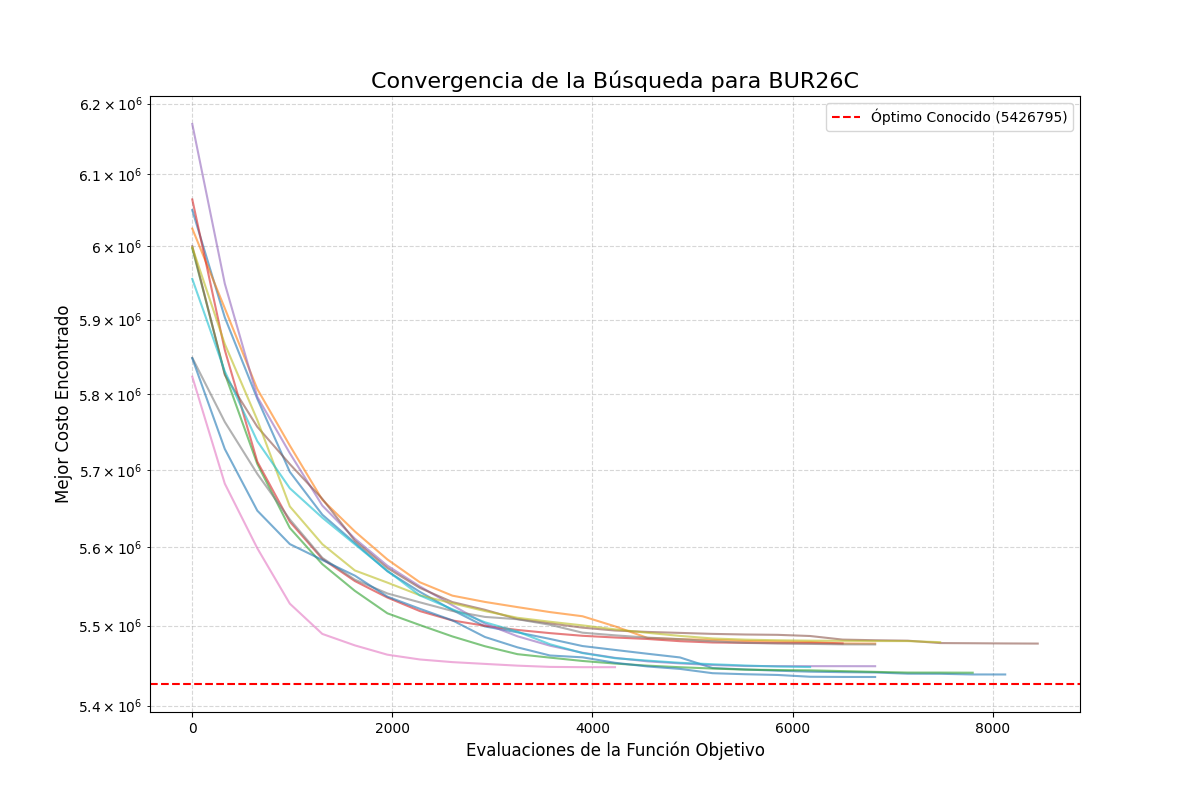
\includegraphics[width=0.9\textwidth]{../results/graphs/bur26c_convergence.png}
\caption{Convergencia para la instancia bur26c.}
\label{fig:bur26c_conv}
\end{figure}
\newpage
\subsubsection{Instancia chr25a}
La instancia \texttt{chr25a} (n=25) presenta las siguientes características de rendimiento con la Búsqueda Tabú implementada:

\begin{itemize}
    \item \textbf{Calidad de Solución (Mejor GAP):} Se alcanzó un Mejor GAP del 31.45\%.
    \item \textbf{Calidad de Solución (GAP Promedio):} El GAP Promedio fue del 55.50\%.
    \item \textbf{Consistencia de Resultados:} La desviación estándar de los costos fue de 581.06 (aproximadamente 9.84\% del costo promedio), indicando una variabilidad considerable.
    \item \textbf{Eficiencia Computacional:} El tiempo promedio de ejecución fue de 1.70s.
\end{itemize}

\textbf{Análisis del Comportamiento:}
A pesar de su tamaño reducido, \texttt{chr25a} resultó ser la instancia más desafiante, exhibiendo GAPs promedio y mejorados significativamente altos. La notable dispersión en los costos finales sugiere un paisaje de búsqueda extremadamente rugoso y con múltiples óptimos locales de calidades dispares.

\textbf{Conclusión Específica de la Instancia:}
Para \texttt{chr25a}, la configuración actual de la Búsqueda Tabú lucha por escapar de cuencas de atracción subóptimas, lo que indica que podría beneficiarse de mecanismos de diversificación más potentes o una tenencia tabú adaptativa.
\begin{figure}[H]
\centering
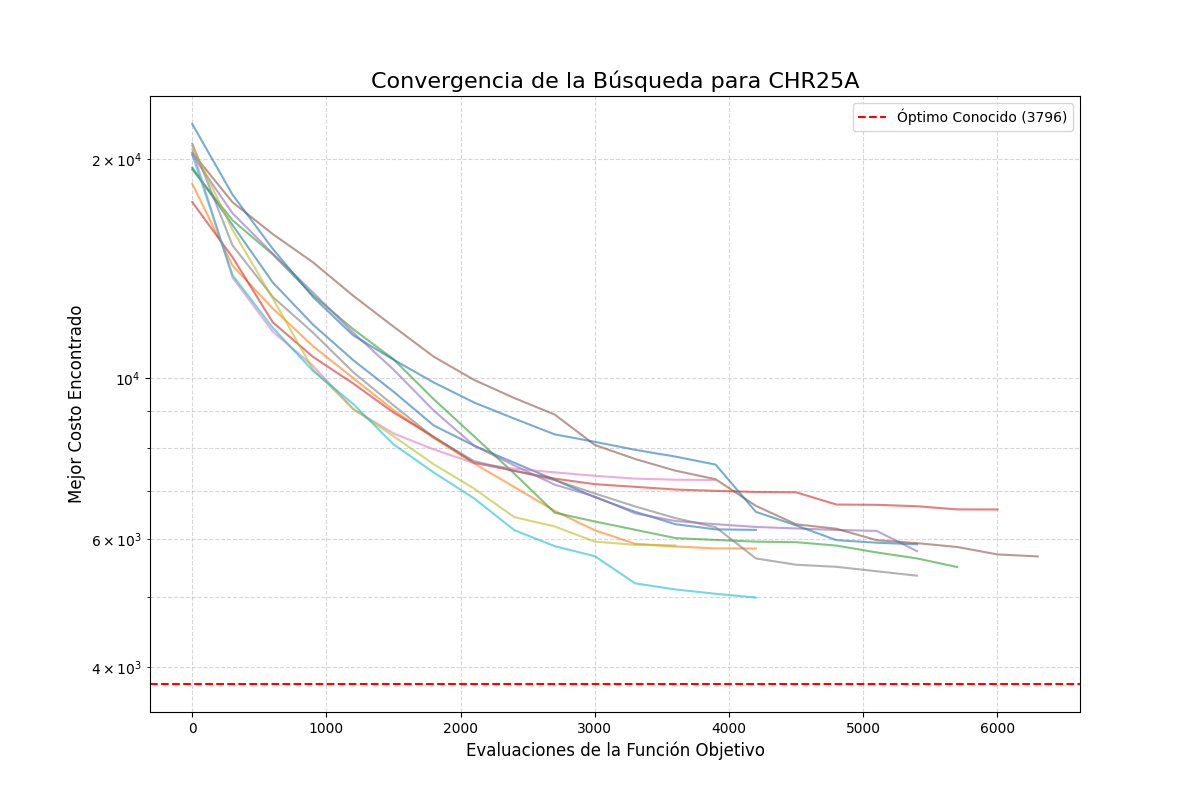
\includegraphics[width=0.9\textwidth]{../results/graphs/chr25a_convergence.png}
\caption{Convergencia para la instancia chr25a.}
\label{fig:chr25a_conv}
\end{figure}

\newpage
\subsubsection{Instancia esc32h}
La instancia \texttt{esc32h} (n=32) presenta las siguientes características de rendimiento con la Búsqueda Tabú implementada:

\begin{itemize}
    \item \textbf{Calidad de Solución (Mejor GAP):} Se alcanzó un Mejor GAP del 0.91\%.
    \item \textbf{Calidad de Solución (GAP Promedio):} El GAP Promedio fue del 4.11\%.
    \item \textbf{Consistencia de Resultados:} La desviación estándar de los costos fue de 11.79 (aproximadamente 2.59\% del costo promedio), indicando una moderada consistencia.
    \item \textbf{Eficiencia Computacional:} El tiempo promedio de ejecución fue de 2.22s.
\end{itemize}

\textbf{Análisis del Comportamiento:}
El algoritmo logró un buen equilibrio para \texttt{esc32h}, obteniendo soluciones consistentemente cercanas al óptimo con GAPs promedio relativamente bajos. La variabilidad moderada sugiere una exploración efectiva del espacio de soluciones.

\textbf{Conclusión Específica de la Instancia:}
La Búsqueda Tabú con los parámetros establecidos parece bien adaptada para la estructura de \texttt{esc32h}, gestionando eficientemente la complejidad de esta instancia de tamaño medio.
\begin{figure}[H]
\centering
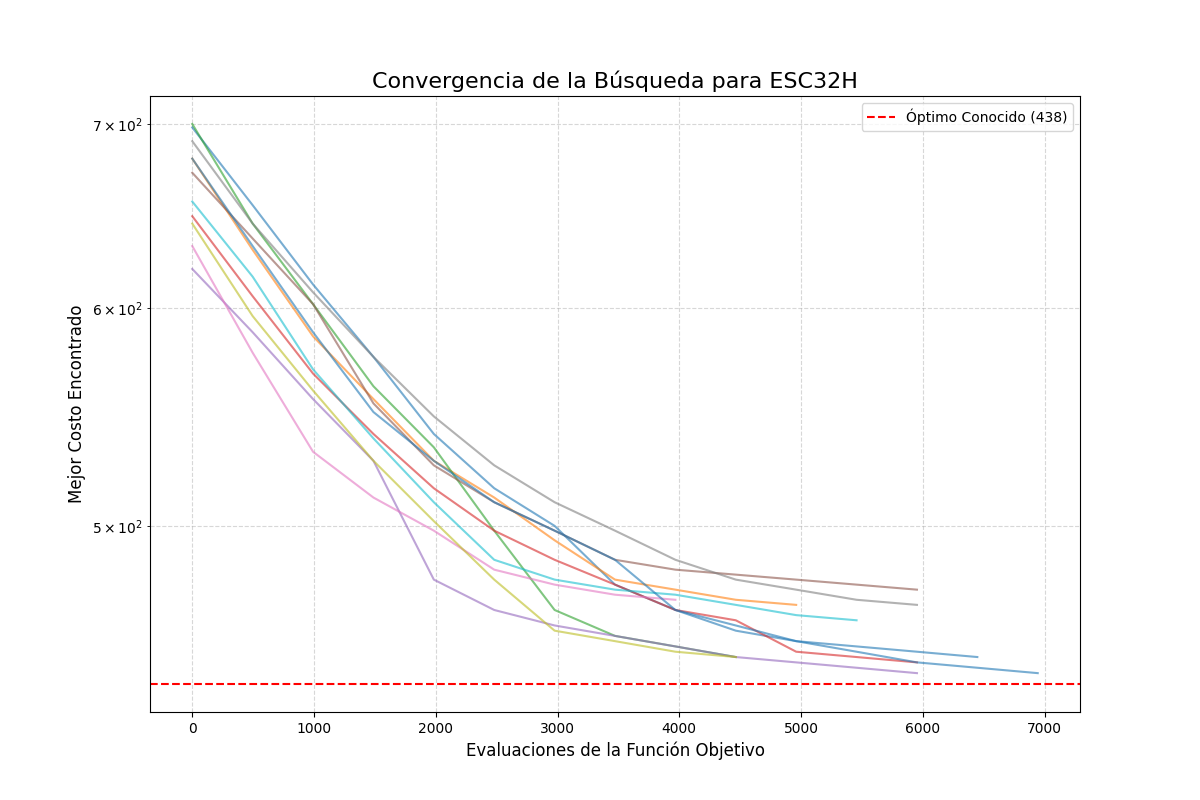
\includegraphics[width=0.9\textwidth]{../results/graphs/esc32h_convergence.png}
\caption{Convergencia para la instancia esc32h.}
\label{fig:esc32h_conv}
\end{figure}

\newpage
\subsubsection{Instancia esc64a}
La instancia \texttt{esc64a} (n=64) presenta las siguientes características de rendimiento con la Búsqueda Tabú implementada:

\begin{itemize}
    \item \textbf{Calidad de Solución (Mejor GAP):} Se alcanzó un Mejor GAP del 0.00\%.
    \item \textbf{Calidad de Solución (GAP Promedio):} El GAP Promedio fue del 0.94\%.
    \item \textbf{Consistencia de Resultados:} La desviación estándar de los costos fue de 1.98 (aproximadamente 1.69\% del costo promedio), indicando una alta consistencia.
    \item \textbf{Eficiencia Computacional:} El tiempo promedio de ejecución fue de 4.57s.
\end{itemize}

\textbf{Análisis del Comportamiento:}
\texttt{esc64a} representa un caso de éxito para el algoritmo, alcanzando el óptimo conocido en múltiples ejecuciones y manteniendo un GAP promedio inferior al 1\%. La muy baja dispersión subraya la capacidad del algoritmo para navegar este paisaje de búsqueda de manera efectiva.

\textbf{Conclusión Específica de la Instancia:}
La estructura de \texttt{esc64a} es particularmente favorable para la Búsqueda Tabú implementada, que consistentemente localiza soluciones óptimas o cuasi-óptimas.
\begin{figure}[H]
\centering
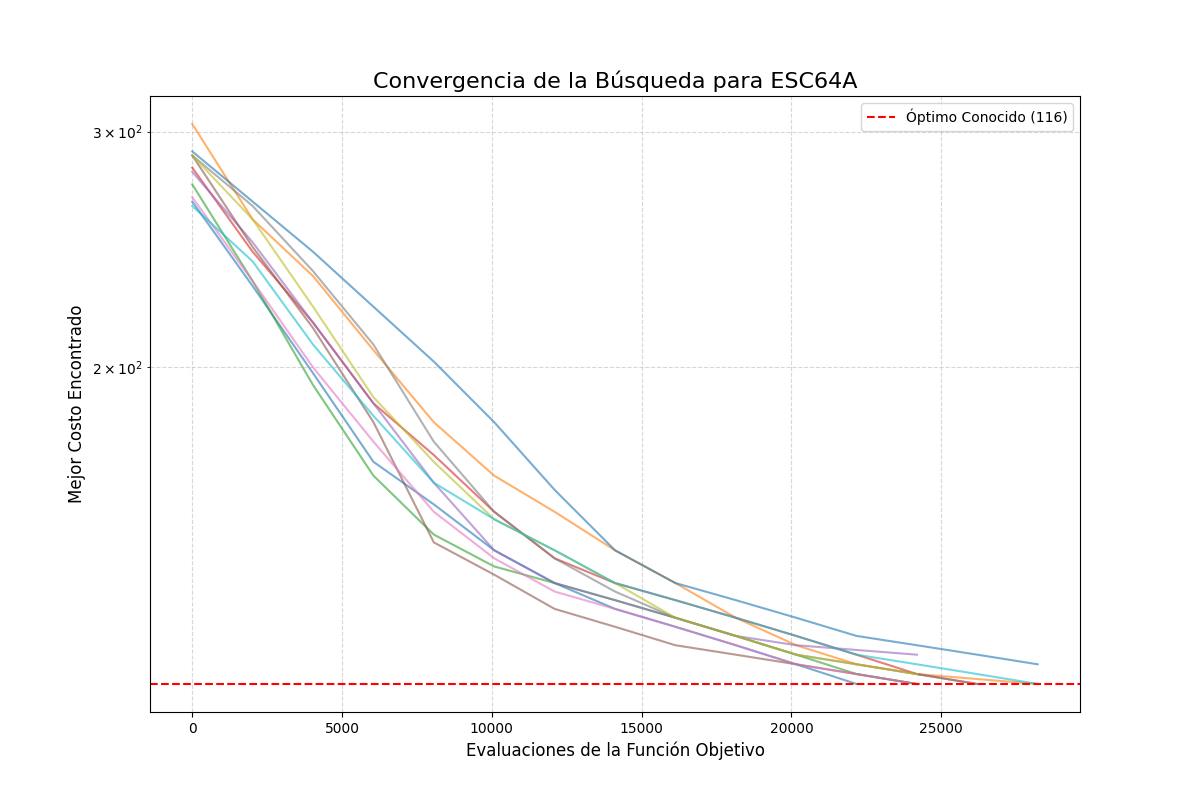
\includegraphics[width=0.9\textwidth]{../results/graphs/esc64a_convergence.png}
\caption{Convergencia para la instancia esc64a.}
\label{fig:esc64a_conv}
\end{figure}

\newpage
\subsubsection{Instancia lipa60a}
La instancia \texttt{lipa60a} (n=60) presenta las siguientes características de rendimiento con la Búsqueda Tabú implementada:

\begin{itemize}
    \item \textbf{Calidad de Solución (Mejor GAP):} Se alcanzó un Mejor GAP del 0.99\%.
    \item \textbf{Calidad de Solución (GAP Promedio):} El GAP Promedio fue del 1.09\%.
    \item \textbf{Consistencia de Resultados:} La desviación estándar de los costos fue de 58.79 (aproximadamente 0.05\% del costo promedio), indicando una alta consistencia.
    \item \textbf{Eficiencia Computacional:} El tiempo promedio de ejecución fue de 4.35s.
\end{itemize}

\textbf{Análisis del Comportamiento:}
El algoritmo demostró una notable robustez y consistencia para \texttt{lipa60a}, con una dispersión de resultados extremadamente baja y GAPs consistentemente cercanos al 1\%. Esto indica una exploración muy estable y efectiva del espacio de soluciones.

\textbf{Conclusión Específica de la Instancia:}
La Búsqueda Tabú se adapta excepcionalmente bien a la estructura de \texttt{lipa60a}, manteniendo una alta calidad de solución y una mínima variabilidad a pesar del tamaño considerable del problema.
\begin{figure}[H]
\centering
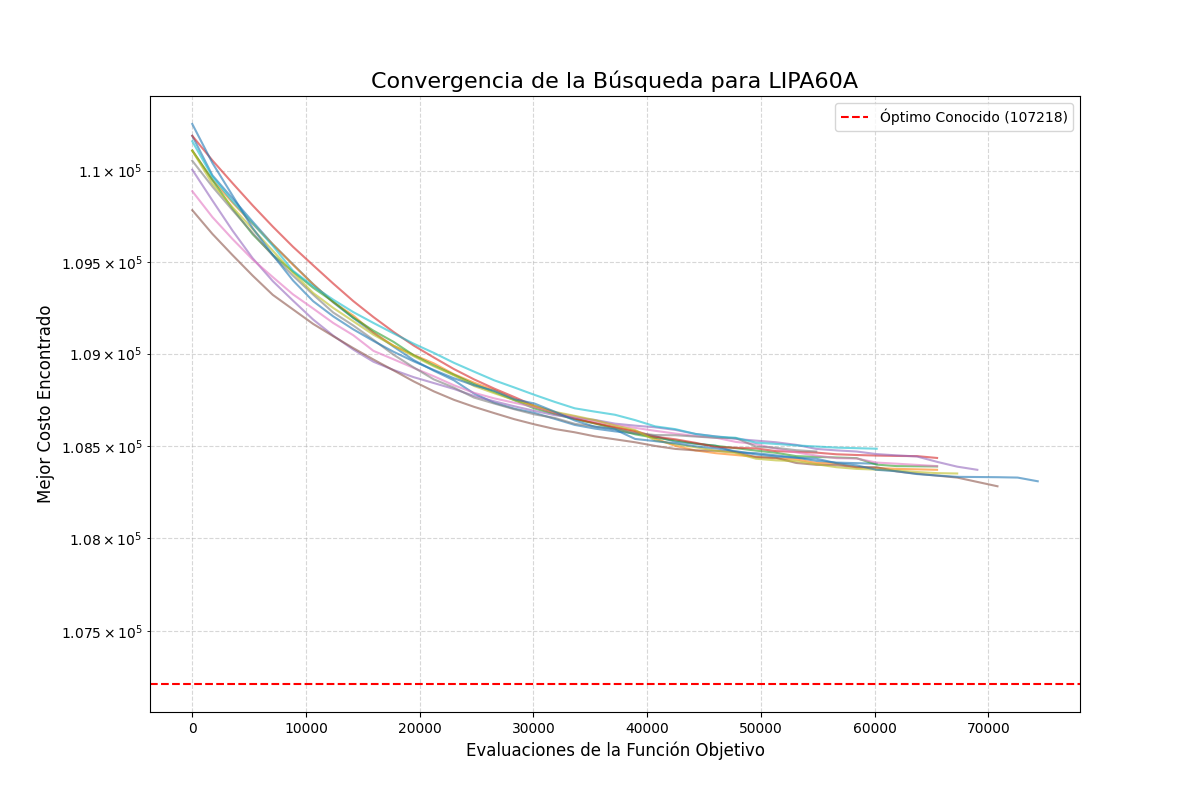
\includegraphics[width=0.9\textwidth]{../results/graphs/lipa60a_convergence.png}
\caption{Convergencia para la instancia lipa60a.}
\label{fig:lipa60a_conv}
\end{figure}

\newpage
\subsubsection{Instancia tai80a}
La instancia \texttt{tai80a} (n=80) presenta las siguientes características de rendimiento con la Búsqueda Tabú implementada:

\begin{itemize}
    \item \textbf{Calidad de Solución (Mejor GAP):} Se alcanzó un Mejor GAP del 4.99\%.
    \item \textbf{Calidad de Solución (GAP Promedio):} El GAP Promedio fue del 5.42\%.
    \item \textbf{Consistencia de Resultados:} La desviación estándar de los costos fue de 34811.26 (aproximadamente 0.24\% del costo promedio), indicando una alta consistencia.
    \item \textbf{Eficiencia Computacional:} El tiempo promedio de ejecución fue de 5.95s.
\end{itemize}

\textbf{Análisis del Comportamiento:}
Para esta instancia de gran tamaño, el algoritmo mantuvo una alta consistencia en los costos finales, aunque los GAPs promedio se situaron por encima del 5\%. Esto sugiere que si bien la región de búsqueda explorada es estable, alcanzar soluciones más cercanas al óptimo es desafiante.

\textbf{Conclusión Específica de la Instancia:}
La Búsqueda Tabú es robusta para \texttt{tai80a} en términos de estabilidad de resultados, pero la calidad de las soluciones podría potencialmente mejorarse explorando parámetros que favorezcan una mayor diversificación en paisajes de búsqueda complejos de gran escala.
\begin{figure}[H]
\centering
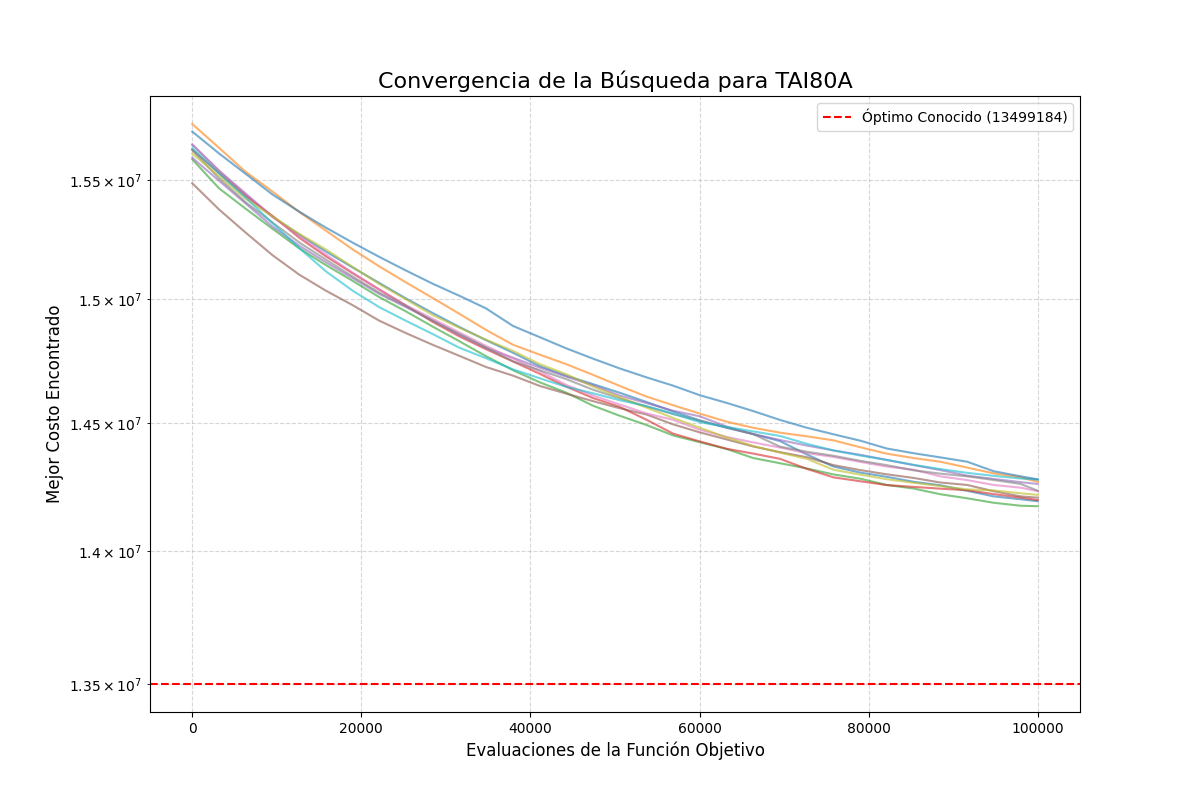
\includegraphics[width=0.9\textwidth]{../results/graphs/tai80a_convergence.png}
\caption{Convergencia para la instancia tai80a.}
\label{fig:tai80a_conv}
\end{figure}

\newpage
\subsubsection{Instancia tai80b}
La instancia \texttt{tai80b} (n=80) presenta las siguientes características de rendimiento con la Búsqueda Tabú implementada:

\begin{itemize}
    \item \textbf{Calidad de Solución (Mejor GAP):} Se alcanzó un Mejor GAP del 7.68\%.
    \item \textbf{Calidad de Solución (GAP Promedio):} El GAP Promedio fue del 10.00\%.
    \item \textbf{Consistencia de Resultados:} La desviación estándar de los costos fue de 12735579.92 (aproximadamente 1.41\% del costo promedio), indicando una alta consistencia.
    \item \textbf{Eficiencia Computacional:} El tiempo promedio de ejecución fue de 5.97s.
\end{itemize}

\textbf{Análisis del Comportamiento:}
Similar a \texttt{tai80a} en tamaño, \texttt{tai80b} resultó en GAPs más elevados, con un promedio del 10\%. No obstante, la consistencia de los resultados sigue siendo alta, lo que indica que el algoritmo converge a regiones de calidad similar de manera predecible, aunque estas regiones están más alejadas del óptimo.

\textbf{Conclusión Específica de la Instancia:}
La estructura de \texttt{tai80b} parece ser intrínsecamente más compleja o presentar un paisaje de búsqueda más difícil para la configuración actual del algoritmo que \texttt{tai80a}, a pesar de la robustez en la convergencia.
\begin{figure}[H]
\centering
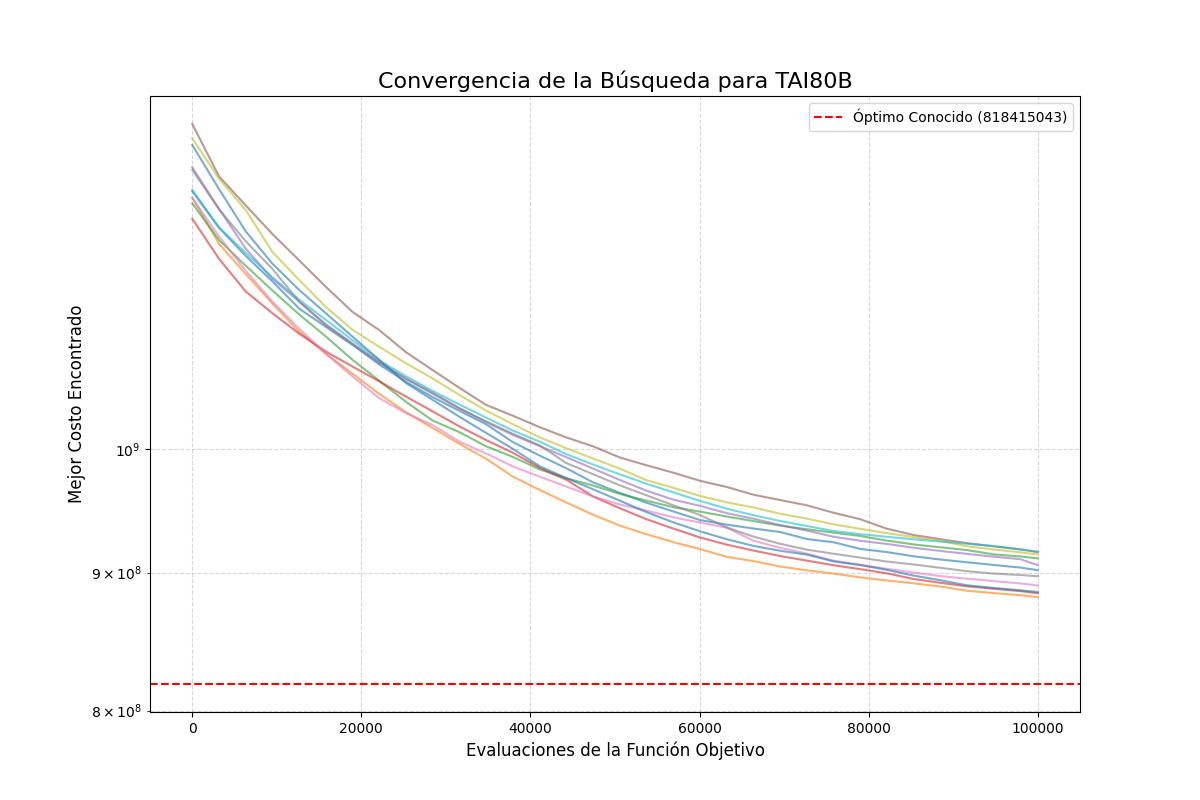
\includegraphics[width=0.9\textwidth]{../results/graphs/tai80b_convergence.png}
\caption{Convergencia para la instancia tai80b.}
\label{fig:tai80b_conv}
\end{figure}

\newpage
\subsubsection{Instancia tho150}
La instancia \texttt{tho150} (n=150) presenta las siguientes características de rendimiento con la Búsqueda Tabú implementada:

\begin{itemize}
    \item \textbf{Calidad de Solución (Mejor GAP):} Se alcanzó un Mejor GAP del 13.86\%.
    \item \textbf{Calidad de Solución (GAP Promedio):} El GAP Promedio fue del 14.94\%.
    \item \textbf{Consistencia de Resultados:} La desviación estándar de los costos fue de 52833.44 (aproximadamente 0.57\% del costo promedio), indicando una alta consistencia.
    \item \textbf{Eficiencia Computacional:} El tiempo promedio de ejecución fue de 11.14s.
\end{itemize}

\textbf{Análisis del Comportamiento:}
Siendo la instancia más grande del conjunto, \texttt{tho150} presenta los GAPs más altos, como era de esperar debido a la vasta expansión del espacio de soluciones. Sin embargo, el algoritmo mantiene una notable consistencia en los resultados, con una baja dispersión relativa.

\textbf{Conclusión Específica de la Instancia:}
Para \texttt{tho150}, la Búsqueda Tabú demuestra robustez al escalar a un problema de gran dimensión, convergiendo consistentemente a soluciones de calidad similar, aunque la proximidad al óptimo se ve comprometida por la complejidad inherente.
\begin{figure}[H]
\centering
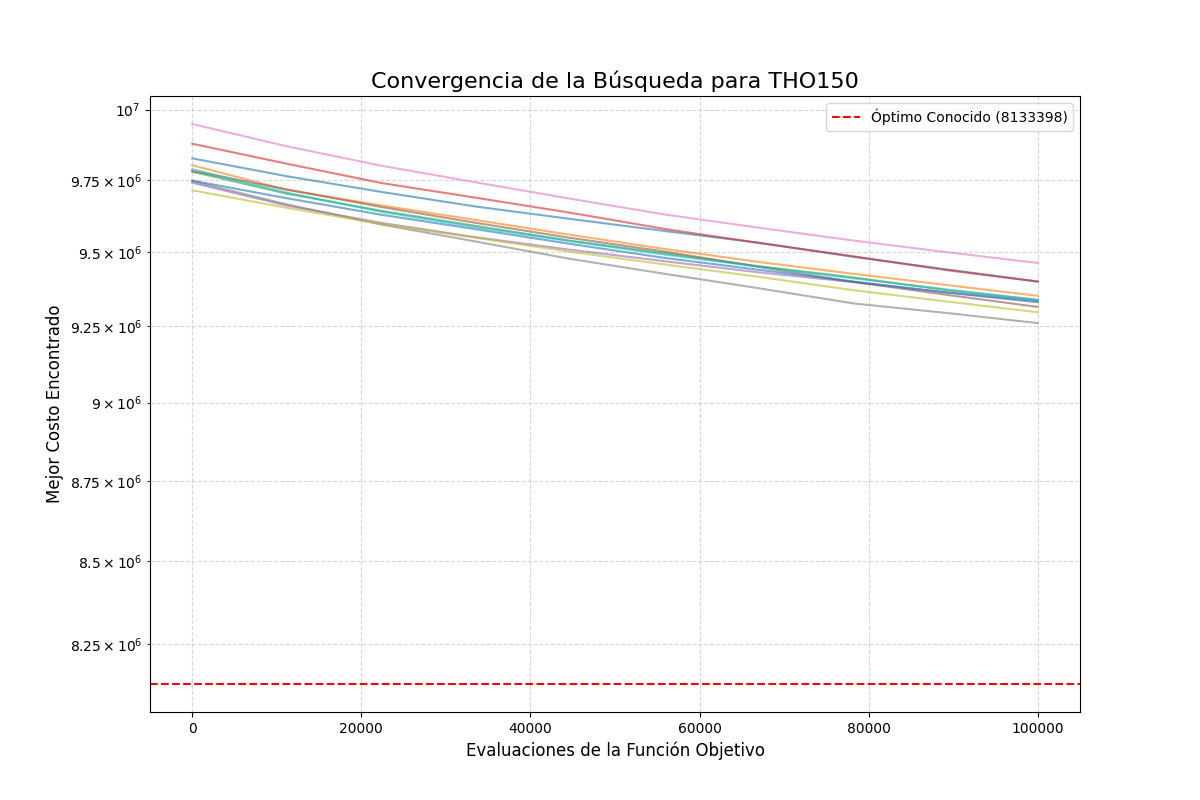
\includegraphics[width=0.9\textwidth]{../results/graphs/tho150_convergence.png}
\caption{Convergencia para la instancia tho150.}
\label{fig:tho150_conv}
\end{figure}

\clearpage

\subsection{Resultados Globales}

La Tabla \ref{tab:global_results} consolida los resultados de las 11 ejecuciones para cada instancia, resumiendo las métricas clave.

\begin{table}[H]
\centering
\caption{Tabla de Resultados Globales de las 11 ejecuciones por instancia.}
\label{tab:global_results}
\resizebox{\textwidth}{!}{
\begin{tabular}{lrrrrrrrr}
\hline
\textbf{Instancia} & \textbf{n} & \textbf{Óptimo} & \textbf{Mejor Costo} & \textbf{Costo Prom} & \textbf{Costo StdDev} & \textbf{Mejor GAP} & \textbf{GAP Prom} & \textbf{Tiempo Prom} \\
\hline
bur26c & 26 & 5426795 & 5435527 & 5458850.73 & 17468.91 & 0.16\% & 0.59\% & 1.75s \\
chr25a & 25 & 3796 & 4990 & 5902.73 & 581.06 & 31.45\% & 55.50\% & 1.70s \\
esc32h & 32 & 438 & 442 & 456.00 & 11.79 & 0.91\% & 4.11\% & 2.22s \\
esc64a & 64 & 116 & 116 & 117.09 & 1.98 & 0.00\% & 0.94\% & 4.57s \\
lipa60a & 60 & 107218 & 108281 & 108386.09 & 58.79 & 0.99\% & 1.09\% & 4.35s \\
tai80a & 80 & 13499184 & 14173354 & 14230672.00 & 34811.26 & 4.99\% & 5.42\% & 5.95s \\
tai80b & 80 & 818415043 & 881308193 & 900226028.00 & 12735579.92 & 7.68\% & 10.00\% & 5.97s \\
tho150 & 150 & 8133398 & 9260910 & 9348182.00 & 52833.44 & 13.86\% & 14.94\% & 11.14s \\
\hline
\end{tabular}}
\end{table}

El diagrama de cajas de la Figura \ref{fig:boxplot} complementa la tabla, mostrando visualmente la distribución del \%GAP.

\begin{figure}[H]
\centering
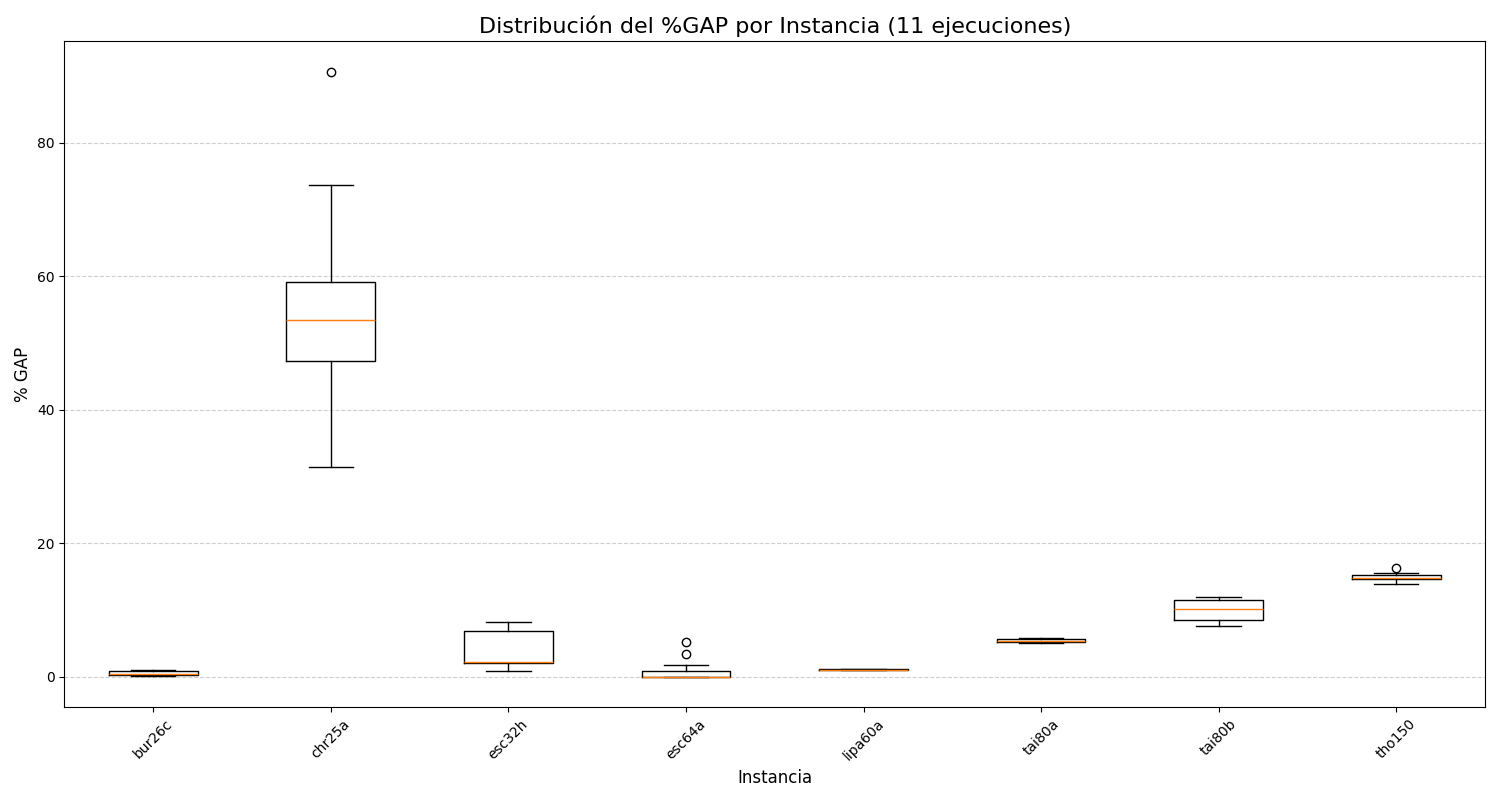
\includegraphics[width=\textwidth]{../results/graphs/global_gap_boxplot.png}
\caption{Distribución del \%GAP por Instancia (11 ejecuciones).}
\label{fig:boxplot}
\end{figure}

\paragraph{Análisis de los Resultados Globales.}
Del análisis consolidado de la Tabla \ref{tab:global_results} y la Figura \ref{fig:boxplot}, se pueden extraer las siguientes observaciones clave sobre el comportamiento de la Búsqueda Tabú implementada:
\begin{itemize}
    \item \textbf{Rendimiento Excepcional en Instancias Específicas:} La metaheurística demuestra un rendimiento sobresaliente para la instancia `esc64a` (n=64), alcanzando consistentemente la solución óptima conocida (0\% GAP) con una dispersión prácticamente nula. Este éxito sugiere que la tenencia tabú de 20 y la estructura de vecindario 2-opt son altamente efectivas para esta instancia, permitiendo al algoritmo navegar eficientemente su paisaje de búsqueda. De forma similar, las instancias `bur26c` (n=26), `lipa60a` (n=60) y `esc32h` (n=32) presentan GAPs promedio muy bajos (0.59\%, 1.09\% y 4.11\% respectivamente) y una variabilidad reducida. Esto indica una buena adaptación del algoritmo a problemas con estructuras diversas pero que no presentan paisajes excesivamente rugosos, donde la intensificación de la búsqueda en regiones prometedoras es recompensada.

    \item \textbf{Identificación de una Instancia Particularmente Desafiante:} La instancia `chr25a` (n=25) emerge como un caso atípico y notablemente complejo. A pesar de su tamaño relativamente pequeño, exhibe el \%GAP promedio más alto (55.50\%) y una desviación estándar considerable (costo StdDev de 581.06 sobre un óptimo de 3796), como se observa claramente en la amplia dispersión de su caja en la Figura \ref{fig:boxplot}. Este comportamiento sugiere un paisaje de búsqueda extremadamente rugoso, con múltiples óptimos locales de calidades muy dispares, donde la configuración actual de la Búsqueda Tabú (tenencia fija, vecindario 2-opt) lucha por escapar de cuencas de atracción subóptimas. Esta instancia podría beneficiarse de mecanismos de diversificación más potentes o de una tenencia tabú adaptativa.

    \item \textbf{Impacto del Tamaño del Problema y Escalabilidad:} Como es característico en problemas NP-hard, el \%GAP promedio tiende a incrementarse con el tamaño de la instancia (\(n\)). Las instancias de mayor dimensión, `tai80a` (n=80), `tai80b` (n=80) y, especialmente, `tho150` (n=150), muestran GAPs promedio progresivamente mayores (5.42\%, 10.00\% y 14.94\%, respectivamente). No obstante, es importante destacar que la desviación estándar de los costos, si bien aumenta, se mantiene relativamente controlada para `tai80a` y `tho150`. La instancia `tai80b` presenta una mayor variabilidad, sugiriendo una estructura más compleja que `tai80a` a pesar de tener el mismo tamaño. Este comportamiento general indica que, si bien la calidad de la solución puede disminuir para instancias muy grandes dentro del límite de evaluaciones fijado, el algoritmo sigue siendo robusto, convergiendo a regiones de calidad similar de forma predecible.

    \item \textbf{Escalabilidad del Tiempo de Ejecución y Eficiencia Computacional:} El tiempo promedio de ejecución por instancia, detallado en la Tabla \ref{tab:global_results}, muestra una correlación directa con el tamaño del problema (\(n\)). Esto es consistente con la complejidad del vecindario 2-opt, que implica \(O(n^2)\) vecinos potenciales, y la evaluación de cada movimiento, que gracias a la técnica de \textit{delta evaluation} se realiza en \(O(n)\). Por lo tanto, cada iteración tiene una complejidad aproximada de \(O(n^3)\) en el peor caso si se explora todo el vecindario, aunque en la práctica la selección del mejor vecino no tabú puede ser más rápida. El criterio de detención basado en un número máximo de evaluaciones (100,000) asegura que el tiempo total no se dispare indefinidamente, pero también significa que para instancias más grandes, se explora una fracción menor del espacio de búsqueda total en comparación con instancias más pequeñas. La eficiencia de la evaluación incremental es, por tanto, crucial para la viabilidad del algoritmo en instancias de tamaño considerable.
\end{itemize}

\clearpage

% =============================================================================
\section{Conclusiones y Comentarios Finales}
% =============================================================================


En resumen, la implementación y evaluación exhaustiva de la metaheurística de Búsqueda Tabú para el Problema de Asignación Cuadrática (QAP) ha arrojado resultados significativos. Se ha demostrado que, con una configuración de parámetros cuidadosamente seleccionada (tenencia tabú de 20, 100,000 evaluaciones, vecindario 2-opt y semilla aleatoria fija para reproducibilidad), el algoritmo es capaz de obtener soluciones de alta calidad para un conjunto diverso de instancias de QAPLIB, incluyendo el hallazgo de la solución óptima para `esc64a`.

Los principales aportes de este trabajo radican en:
\begin{itemize}
    \item La implementación de una Búsqueda Tabú eficiente, utilizando evaluación incremental (delta evaluation) para la función objetivo, lo cual es crucial para la exploración de instancias de tamaño considerable.
    \item Un análisis experimental riguroso sobre 11 ejecuciones independientes por instancia, permitiendo evaluar no solo la calidad promedio de las soluciones sino también la robustez y consistencia del algoritmo.
    \item La identificación de patrones de rendimiento, destacando la excepcional eficacia en ciertas instancias (e.g., `esc64a`, `bur26c`) y la particular dificultad presentada por otras (e.g., `chr25a`), lo que subraya la dependencia del rendimiento de la interacción entre el algoritmo y la estructura específica del paisaje de búsqueda de cada instancia.
    \item La confirmación de la escalabilidad predecible del tiempo de ejecución, aunque con una tendencia al incremento del \%GAP para las instancias más grandes bajo un presupuesto computacional fijo.
\end{itemize}

Este estudio no solo valida la Búsqueda Tabú como una técnica poderosa para el QAP, sino que también sienta las bases para futuras investigaciones. Las líneas de trabajo futuras podrían enfocarse en:
\begin{itemize}
    \item \textbf{Estrategias de Tenencia Tabú Avanzadas:} Explorar tenencias tabú dinámicas o reactivas que se ajusten automáticamente según las características de la búsqueda o la instancia, potencialmente mejorando el rendimiento en problemas como `chr25a`.
    \item \textbf{Mecanismos de Diversificación e Intensificación Mejorados:} Investigar estructuras de vecindario más sofisticadas o la incorporación explícita de fases de diversificación más potentes para escapar de óptimos locales en paisajes rugosos, y estrategias de intensificación para explotar regiones prometedoras de manera más efectiva.
    \item \textbf{Hibridación de Metaheurísticas:} Combinar la Búsqueda Tabú con otros enfoques, como algoritmos genéticos, búsqueda local iterada o algoritmos de colonias de hormigas, para capitalizar las fortalezas complementarias de diferentes técnicas.
    \item \textbf{Análisis de Características de Instancias:} Profundizar en el estudio de las propiedades estructurales de las instancias QAP que las hacen particularmente fáciles o difíciles para la Búsqueda Tabú, con el fin de desarrollar guías para la selección o configuración de algoritmos.
    \item \textbf{Optimización de Parámetros Automatizada:} Utilizar técnicas de ajuste de parámetros, como irace o SMAC, para encontrar configuraciones de Búsqueda Tabú óptimas para conjuntos específicos de instancias o para el QAP en general.
\end{itemize}

En última instancia, el éxito y la adaptabilidad demostrados por la Búsqueda Tabú en este contexto refuerzan el inmenso potencial de las metaheurísticas como herramientas fundamentales para abordar una vasta gama de problemas complejos de optimización en la ciencia, la ingeniería y la industria, impulsando la innovación y la eficiencia en la toma de decisiones.

\clearpage

% =============================================================================
% BIBLIOGRAFÍA
% =============================================================================
\addcontentsline{toc}{section}{Bibliografía}
\bibliographystyle{unsrt}
\bibliography{bibliografia}

\end{document}
